% Setup - do not change
\documentclass[11pt]{article}
\usepackage[top=0.9in, left=0.9in, bottom=0.9in, right=0.9in]{geometry} 
\usepackage{parskip}

\usepackage[english]{babel}
\usepackage[utf8]{inputenc}
\usepackage{amsmath,amsthm,amssymb,graphicx,pdfpages,lipsum,hyperref}
\usepackage[none]{hyphenat}
\usepackage{csquotes}

\setlength\parindent{0pt}
%%%%%%%%%%%%%%%%%%%%%%%%%%%%%%%%%%%%%%%%%%%%%%%%%%%%%%%%%%%%%%%%%%%
% add other packages here if required

\usepackage[sorting = none]{biblatex}
\addbibresource{references.bib}


\title{\textbf{Demand Estimation for Trips from JFK Airports} \\ {New York Yellow Taxi}}
\author{
Patrick Lourenz \\
Student ID: 1470744 \\
%% Replace the link with your github repo
% 1. Remember to escape underscore (\_) in the link.
% 2. Remember to include the commit you want to submit in the link
\href{https://github.com/MAST30034-Applied-Data-Science/mast30034-project-1-pl0203/commit/eea592dc589340d50c9e1d20522327cdd9c7723d}{GitHub repository with commit}
}

\begin{document}
\maketitle

\section{Introduction}
% Link to a 30 min tutorial if you require revision: https://www.overleaf.com/learn/latex/Learn_LaTeX_in_30_minutes

Yellow taxis have been very closely acquainted with the city of New York. However, New York City Taxi and Limousine Commission (TLC) has been struggling since ride-sharing like Uber and Lyft disrupted the marketplace. It is evident with the decreasing taxi cab medallion licenses. There were 51,398 active taxi licenses as of March 2014. As of July 2016, this number has dropped significantly to 13,587 \cite{taxi1}. 

\\
Substantively, taxis still do have an advantage over ride-share services. When demand is higher than supply for ride-share services, this can benefit taxis as there is a high chance that the price will be more affordable to take a taxi. Uber and Lyft, utilise demand spikes to formulate dynamic surge prices whereas NYC taxis do not have a surge pricing mechanism \cite{taxistrive}. Therefore, TLC needs to be able to meet demand at certain time and strategic location, such as JFK Airport.  

\\
This report will analyse and predict from the viewpoint of a taxi company. As the data reflect users' behaviour, the aim is to assist this company to understand the marketplace behaviour in JFK Airport and be able to fulfil supply in specific hours utlising the estimated demand. The Prediction used a Multiple Linear Regression model, as a base model \cite{mlr}, and a Random Forest Regression model \cite{rf}. Random Forest Regression was used as it is expected to be able to capture complex decision boundaries and relationships between features through multiple decision trees majority voting.
\\

\section{Dataset}
\subsection{Yellow Taxi Trip Record}
This report fundamentally used the monthly \textbf{Yellow Taxi Trip Record} dataset released by New York TLC from \textbf{2018-2019}\cite{nyctaxi}. In March 2020, New York City went into lockdown. This certainly impacted taxi demand negatively. Therefore, this report did not include trip data from 2020 and beyond. Green Taxi Trip Record was not included in this report as they are not allowed to pick up passengers from airports. 

Initially, this dataset contains 187,469,831 rows and 19 columns. However, after cleaning and selecting relevant features dataset was reduced to 10,308,204 rows and for the purpose of this report, five columns were selected; \textbf{Pick-up Date and Time, Drop-off Date and Time, Pick-up Location ID, and Drop-off Location ID}. 

\subsection{JFK Airport's hourly observed weather data}
Supporting the trip dataset, external datasets were also included. The first dataset was JFK Airport's hourly observed weather data from 2018-2019 retrieved from United States National Centers for Environmental Information (NCEI)\cite{weather}. This data has 27,170 rows and for the purpose of this report seven columns were selected; \textbf{Date and Time, Temperature, Dew Point, Precipitation, Wind Direction, Pressure, and Visibility}.

\subsection{New York Public School Holiday}
Another external dataset included was the New York Public School Holiday from 2018-2019 retrieved from the New York Department of Education website \cite{school}. Hypothetically, the school holidays may increase airport pickup demand as more people travel to New York for vacation purposes, assuming most cities have the same holiday dates. Moreover, approaching the end of a long school holiday, \textit{New Yorkers} will return to their city. This, expectedly, will also increase airport pickup demand. 

\section{Preprocessing}
\subsection{Yellow Taxi Data (Outlier Detection)}
\noindent\textbf{Out of range pick-up dates}
\\
There were trips with pick-up date outside of the selected year 2018 and 2019. These data were filtered out.

\noindent\textbf{Negative trip duration}
\\
There were trips where pick-up date timed after the drop-off date, intuitively this is not possible. These data were removed.

\noindent\textbf{Trips with duration more than 5 hours}
\\
A trip from JFK, LaGuardia or Newark Airport to the furthest point destination in New York during peak afternoon hours is estimated by Google Maps to take 1.5 - 2 hours. According to the New York TLC, drivers are not permitted to refuse passengers with more than one stop (taximeter will run as one continuous trip). Therefore, trips that have more than 5 hours (3 hours added to assume multiple stops trip) in trip duration were eliminated.

\noindent\textbf{Only trips from airports}
\\
As the report aim is to estimate demand from airports, only trips from Newark, JFK, or LaGuardia Airport were selected.

\noindent\textbf{Check for null values}
\\
After previous filter steps taken, there were no more null values present in the taxi data.

\subsection{Weather Data}
\noindent\textbf{Imputations for missing data}
\\
According to the weather dataset documentation, there are consecutive 9s (i.e. 999.9, 999, 999.0) in the dataset and these were missing values. Therefore, these data were converted to null values.

\noindent\textbf{Imputations for null values}
\\
There are null values across all weather features with precipitation being the most (6,214 rows). Null values were replaced using the median value within a day's 6 hours time frame; 12 AM - 6 AM, 6 AM - 12 PM, 12 PM - 6 PM, 6 PM - 12 AM.

\section{Analysis}
\subsection{Airport is an important location for TLC}
\begin{table}[h]
	\begin{center}
		\begin{tabular}{|l|l|l|}			
			\hline
			2018-2019 & Proportion of Trips & Proportion of Total Amount \\
			\hline\hline
            All Airports Pick-up & 5.51\% & 15.58\% \\
			\hline
			\textbf{JFK Airport Pick-up} & \textbf{2.81\%} & \textbf{9.00\%}\\
			\hline
			Other Airports Pick-up & 2.70\% & 6.58\% \\
			\hline
		\end{tabular}
		\caption{Proportion of Airport Pick-up Trips from all yellow taxi trips in New York 2018-2019}
		\label{table1}
		
	\end{center}
\end{table}
JFK Airport is a strategic location for TLC. This is due to trips from and to the airport being highly valuable. Table ~\ref{table1} describes the proportion of trips from JFK Airport proportion in terms of trip count and total amount. JFK Airport pick-up trip contributed to 2.81\% of the total trips but contributed 9.00\% to the total generated total amount. This explains that JFK airport trips, generally, are high average selling price trips (even higher than other airports).

\subsection{Drop-off Locations}
Figure ~\ref{fig:geo} displays the drop-off locations of yellow taxi trips that started from JFK Airport. It appears that most trips end around the Manhattan area. This is as expected as Manhattan is a tourist destination and Lower Manhattan is the central borough for business. Moreover, TLC charges a flat rate of \$52 for trips between Manhattan and JFK Airport. This could be the reason why people commuting to Manhattan prefer taxis to ride-share. Hence, the demand for a trip to Manhattan from JFK Airport is high.
\\
Interestingly, LaGuardia and JFK Airport itself are also high drop-off locations from JFK Airport. This could be due to transit flights to LaGuardia Airport or between terminal commuting in JFK Airport.
\begin{figure}[h]
    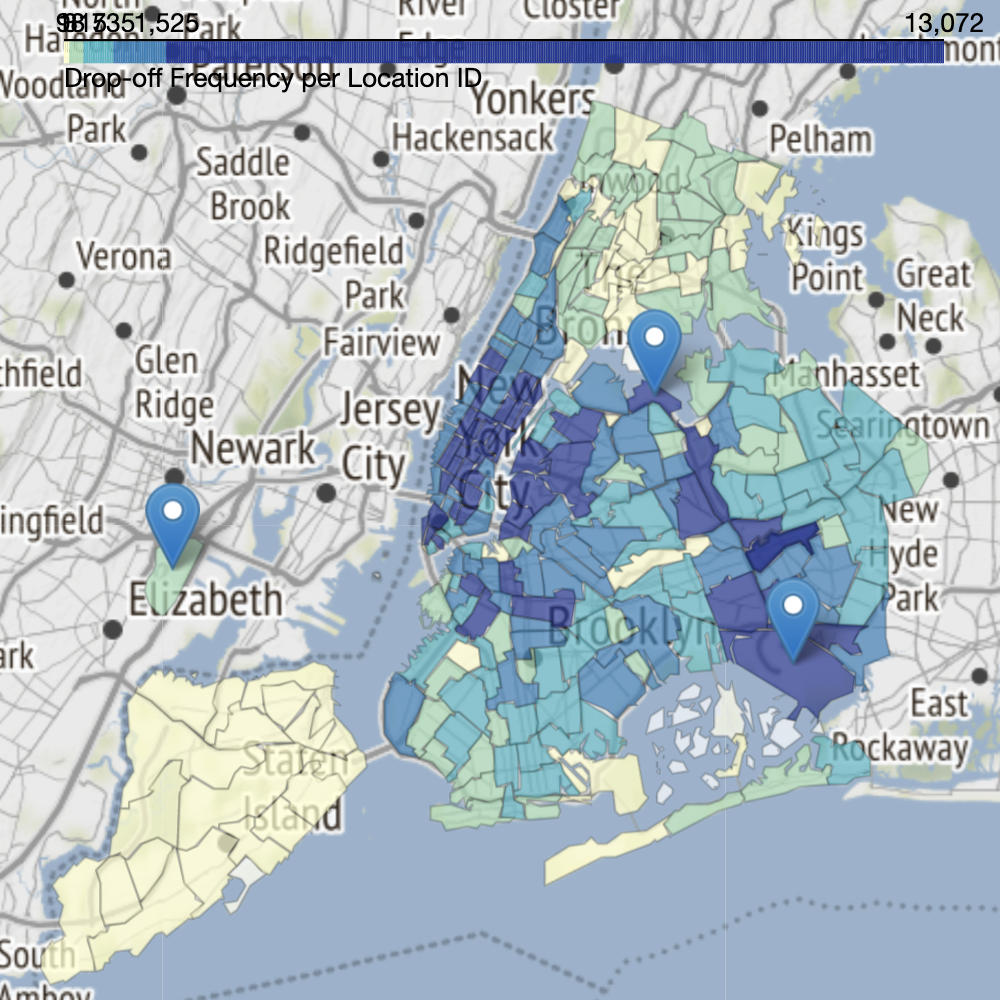
\includegraphics[width=0.4\textwidth]{plots/geospatial_vis.png}
    \centering
    \caption{Drop-off Frequency per Location ID. Markers denote airport locations.} 
    \label{fig:geo}
\end{figure}


\subsection{Correlation between features}
There are clear evidence where there exists strong evidence that features are correlating with each other. For instance, in Figure ~\ref{fig:corr}, it shows a strong correlation between \texttt{temperature} and \texttt{dew\_point}. The p-value between these two features was also lower than 0.05, shown in Figure ~\ref{fig:corr_pval}. Therefore, there is enough evidence that there is a correlation between these two features. These strongly correlated features will be assessed later before modelling.
\begin{figure}[h]
    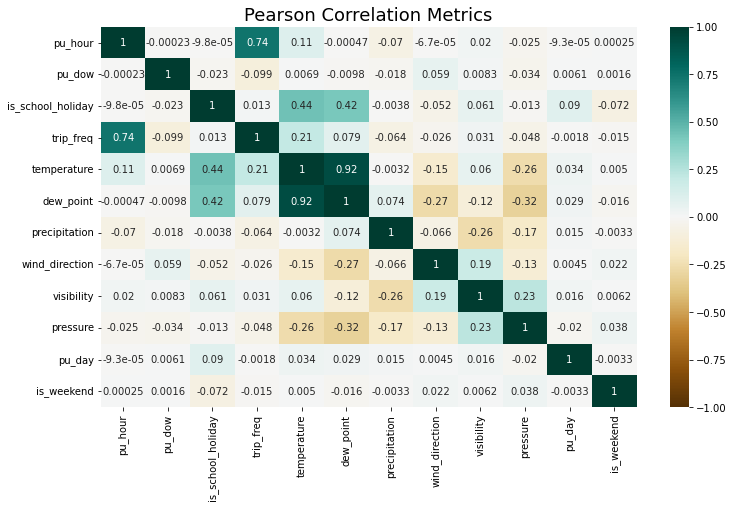
\includegraphics[width=0.7\textwidth]{plots/corr_heatmap.png}
    \centering
    \caption{Pearson Correlation Heat-map between features}
    \label{fig:corr}
\end{figure}
\begin{figure}[h]
    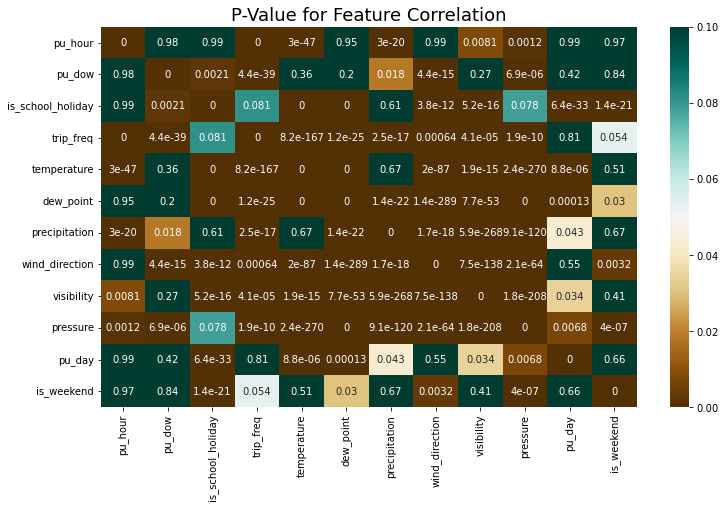
\includegraphics[width=0.6\textwidth]{plots/pval_heatmap.png}
    \centering
    \caption{P-value for Correlation between features}
    \label{fig:corr_pval}
\end{figure}

\subsection{Insight 1: Most airport pick-up ride passengers are business travellers}
The hourly taxi pick-up rate was grouped by day of the week to further analyse the behaviour of users. Figure ~\ref{fig:hour_dow} shows that the median trip frequency shows that Saturdays, in general, have the lowest daily trips, this insight may show that most airport pickup trips are business travellers. Sundays and Mondays are exceptionally high as this day, most business travellers come to start their working week. Tuesday and Wednesday, demand drop is as expected as not many business travellers travel during in the middle of a working week.
\begin{figure}[h]
    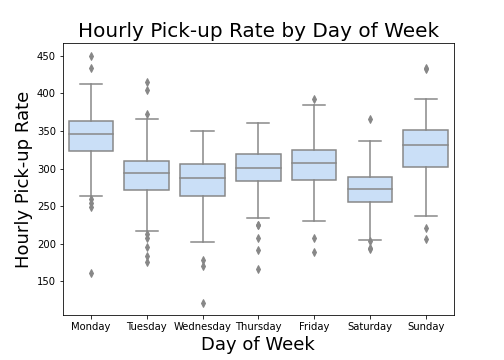
\includegraphics[width=0.55\textwidth]{plots/hourly_pickup_rate_by_dow.png}
    \centering
    \caption{JFK Airport Pick-up Hourly Rate by Day of Week} 
    \label{fig:hour_dow}
\end{figure}


\subsection{Insight 2: Airport pick-up demand peak times in a day}
Figure ~\ref{fig:hour} captured the demand drops and peaks within the hours in a day. Lowest JFK Airport pick-up demand is during graveyard hours, 1 am - 5 am, which is as expected. In contrast, demand spikes multiple times; in the morning (6-7 am), afternoon (2 pm - 5 pm), and night (8 pm - 9 pm).
\begin{figure}[h]
    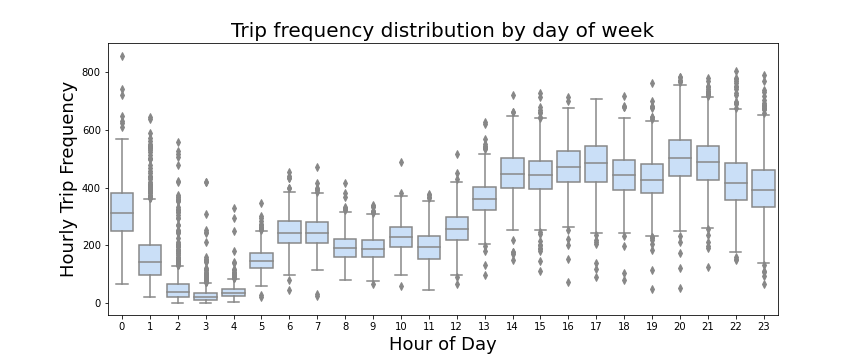
\includegraphics[width=0.9\textwidth]{plots/hourly_pickup_rate.png}
    \centering
    \caption{JFK Airport Pick-up Hourly Rate} 
    \label{fig:hour}
\end{figure}
\subsection{Insight 3: School holidays do impact airport pick-up demand}
School holidays may impact positively or negatively airport pick-up demand. In Figure ~\ref{fig:christmas}, demand was compared between December 25, 2018, and the previous 2 weeks. The result showed that overall demand decreased throughout the day, but spiked at 11 pm.
\begin{figure}[h]
    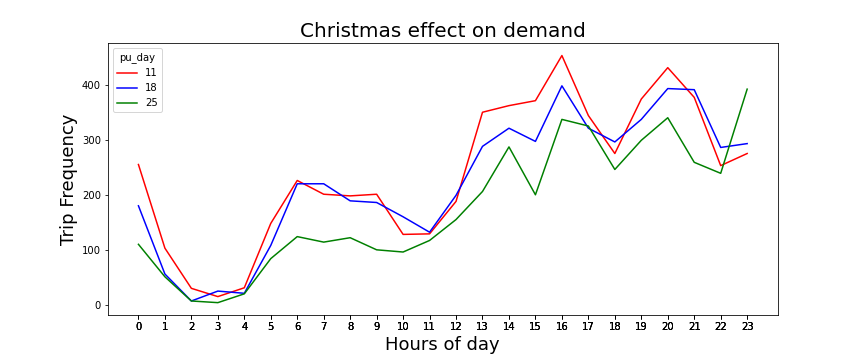
\includegraphics[width=0.8\textwidth]{plots/school_holiday_Christmas.png}
    \centering
    \caption{Christmas Day impact on JFK Airport taxi pick-up demand} 
    \label{fig:christmas}
\end{figure}
\\
Figure ~\ref{fig:summer} visualises when a longer holiday period, such as summer break, was compared to \textit{non-}summer break days. The result was summer break increased airport pick-up demand overall.
\begin{figure}[h]
    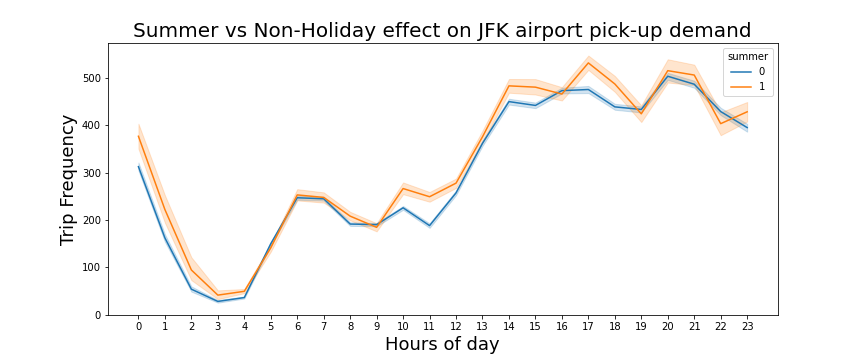
\includegraphics[width=0.85\textwidth]{plots/school_holiday_summer.png}
    \centering
    \caption{Summer break impact on JFK Airport taxi pick-up demand} 
    \label{fig:summer}
\end{figure}

\section{Data Aggregation, Feature Selection and Engineering}
Prior to statistical modelling, taxi dataset are grouped by the date and hour and a new feature, \texttt{trip\_frequency}, aggregates the record count. Next, weather data was merged using inner join to eliminate missing hours. \texttt{is\_school\_holiday} boolean feature was also added to identify if the pick-up date was a school holiday.
Following the correlating features; \texttt{temperature} and \texttt{dew\_point} from the Analysis section, two ordinary least squares (OLS) regressions were fitted to compare which model has the lowest Akaike Information Criterion (AIC) \cite{aic}. The result was the model without \texttt{dew\_point} has the lowest AIC. Therefore, \texttt{dew\_point} was eliminated.

Ordinal features were one-hot encoded and numerical features were standardised to avoid bias introduced to the model.


\section{Statistical Modelling}
Test data used was a yellow taxi, weather and school holiday data from January 2020. It was pre-processed following the same steps as the train data.
\\
Metrics used to assess the model performance are root mean squared error (RMSE), mean absolute percentage error (MAPE), and $R^2$ score. RMSE explains how far off, in terms of the number of trips, the model predictions to the actual target value, while the MAPE described the error in terms of percentage from the actual value. $R^2$ score showed the amount of variability in the data that can be explained by the model.


\subsection{Multiple Linear Regression (baseline model)}
Multiple linear regression enables the model to assess multiple features by conducting linear regression with each feature and the target feature which follows this equation:
\[Y_i = f(X_i, \beta) + e_i\]
The model resulted in an RMSE of 71.48 trips, a MAPE of 30.68\%, and $R^2$ score of 0.8061. These metrics will be used as a baseline for the Random Forest Regression. Considering this linear regression may not capture the complex relationship between features, a $R^2$ score of 0.8061 was a promising sign.

\subsection{Random Forest Regression}
Random forest regression is a supervised machine learning method that ensembles \textbf{\textit{n}} decision trees on various sub-sample of the dataset. A majority vote was then taken from all trees to generate a predicted result.

There are two hyper-parameters; \texttt{max\_features}, \texttt{n\_estimators}. These were tuned by selecting the lowest RMSE and highest $R^2$ score. \texttt{max\_features} and \texttt{n\_estimators} were set to 18 and 300 respectively.

Random forest regression resulted in an MAE of 66.13 trips, MAPE of 26.17\% and $R^2$ score of 0.8344. These metrics were understandably much better than the linear regression results.

Figure ~\ref{fig:rf_hour_pred_act_jan_2020} shows that on most dates, the difference between predicted and actual demand was not far off. The demand spike that the model could not predict was for the 2nd, 5th and 20th of January. It appears that there was an NHL sporting event on the 5th and 20th date, while on the 2nd there was an NBA game. This was further supported with Figure ~\ref{fig:rf_hour_pred_act_20220127} showing the model underestimated 3 consecutive hours, 6 pm - 8 pm. This was when the NHL game began. 

\begin{figure}[h]
    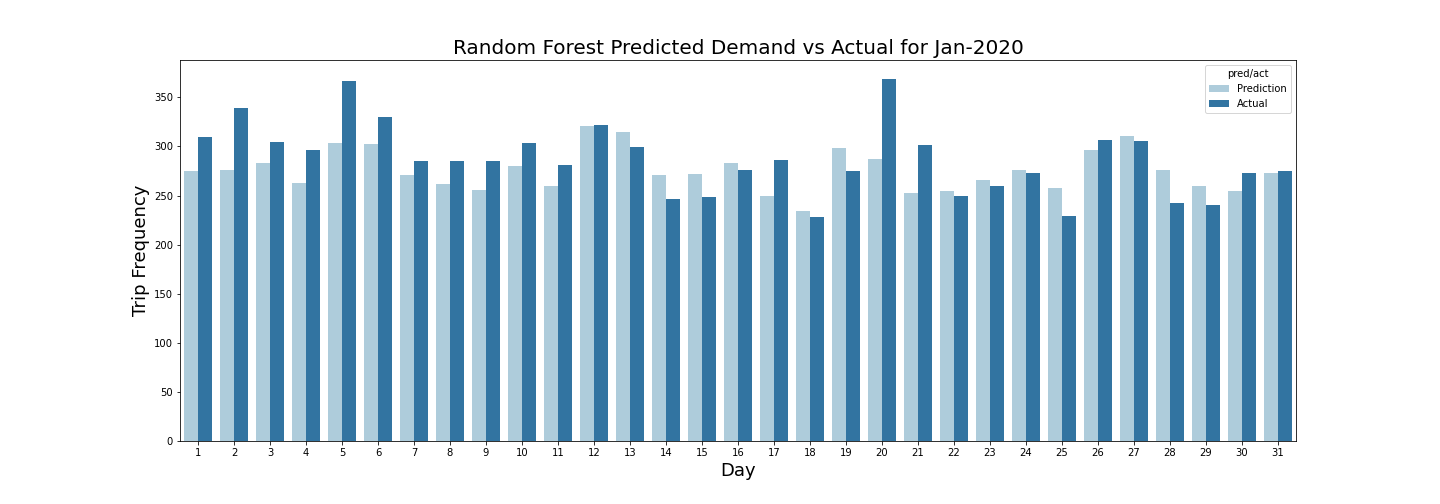
\includegraphics[width=1.0\textwidth,height=5cm]{plots/rf_hour_pred_act_jan_2020.png}
    \centering
    \caption{Random forest regression predicted demand for January 2020} 
    \label{fig:rf_hour_pred_act_jan_2020}
\end{figure}
\begin{figure}[h]
    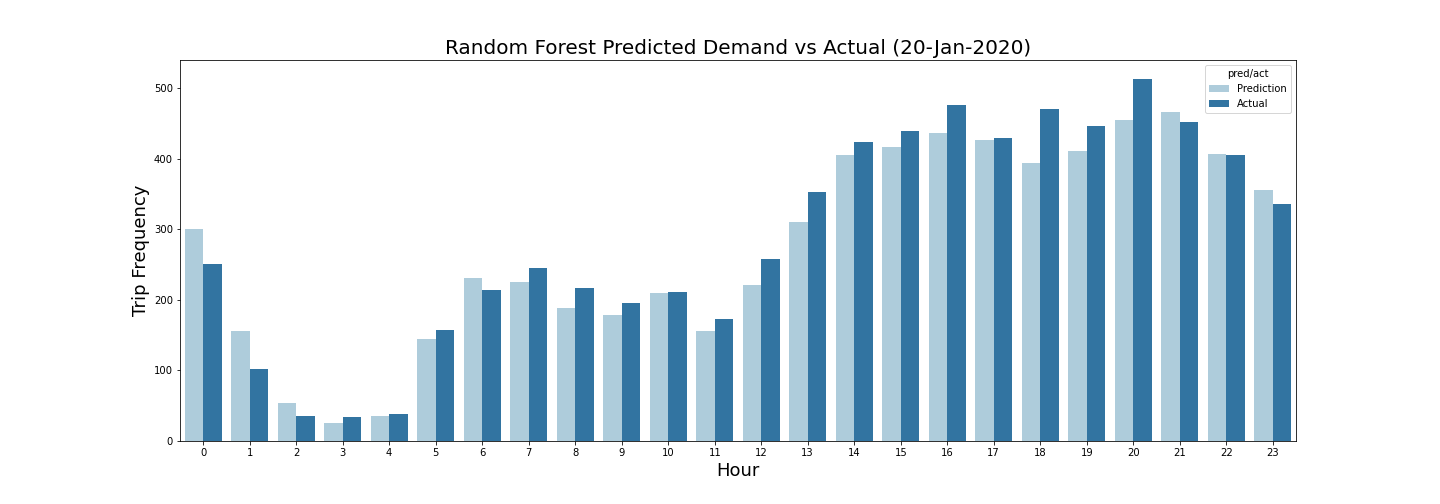
\includegraphics[width=0.9\textwidth,height=5cm]{plots/rf_hour_pred_act_20220120.png}
    \centering
    \caption{Random forest regression predicted demand compared to the actual trips at January 20, 2020} 
    \label{fig:rf_hour_pred_act_20220127}
\end{figure}
\begin{figure}[h]
    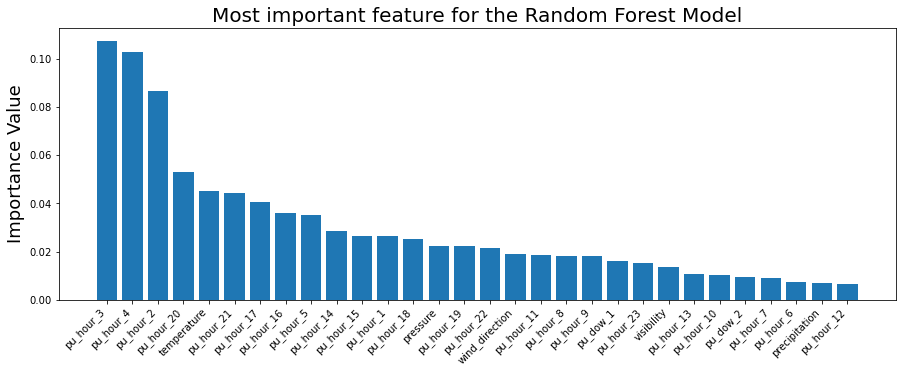
\includegraphics[width=0.9\textwidth]{plots/rf_important_feat.png}
    \centering
    \caption{Important Features according to the Random Forest model} 
    \label{fig:rf_hour_pred_act_20220127}
\end{figure}

\section{Recommendations and Conclusion}
This report has presented how JFK Airport pick-up demand can be estimated using Linear Regression and Random Forest Regression method utilising New York Yellow Taxi dataset, JFK Airport weather dataset, and New York School Holiday. The model error may be slightly too high for TLC to implement this for their decision-making as it has an MAE of 66.13 trips and a MAPE of 26.17\%. In future implementations, more effort should be made in cleaning data outliers for both weather and taxi.
Furthermore, random forest regression performance may need to be compared with other machine learning models that are more sophisticated in terms of understanding the data, such as deep neural networks.

There were demand spikes that the model could not explain, as seen in Figure ~\ref{fig:rf_hour_pred_act_jan_2020}. Most of these dates were where major sporting events were played. Future implementations could add New York major sporting events dates data, such as NHL and NBA. 

Moreover, it can be interesting to investigate how yellow taxi demand influences ride-share demand and vice versa. Moreover, looking deeper into how dynamic price surge ride-share services in conjunction with demand estimation can be beneficial for the New York TLC. This will help them to know where to direct supplies to a specific location at a specific time where taxi price can win over ride-share.




\clearpage

% BEGIN REFERENCES SECTION
\printbibliography

\end{document}